
% vim:set ff=unix expandtab ts=2 sw=2:
\newlength{\mycolwidth}
%\setlength{\mycolwidth}{.48\textwidth} % for 2 columns
\setlength{\mycolwidth}{.31\textwidth} % for 3 columns
% measure the height of the blocks

\begin{columns}
	% -------------
	% SECOND COLUMN
	% -------------
	\begin{column}{\mycolwidth}
		\begin{center}
			%\begin{minipage}[T]{.95\textwidth}
				\parbox[t][\columnheight]{\textwidth}{
						
% vim:set ff=unix expandtab ts=2 sw=2:

\alert{\textit{Positive aspects:}}
\begin{itemize}
    \item The header can contain arbitrary formatting like this one
      but the defaults can be controlled by the template file like the next one.
    \item The box will grow with its content automatically, which is nice
      as long as you do not want to align the top AND the bottom of different boxes.
\end{itemize}
 
\alert{\textit{Problem:}}
Since the size of the boxes is determined by their content it is extremely difficult to align the last box to the bottom of the page
while keeping the top of the first box aligned.
This will only be possibe by ajusting a 
\begin{verbatim}
\vspace{}
\end{verbatim}
In the CONTENT of one of the blocks.
This can be done either by    a manual adjustment after everything else is done (very un \LaTeX like) , or by automatically measuring everything else in the column by using saveboxes around the other content like in the following example.
\begin{verbatim}
\newsavebox\mybox
\setbox0=\vtop{%
		\begin{block}{A standard block} 
			some text  
		\end{block}%
}
\newlength{\bh}
\setlength{\bh}{\ht0}%
\addtolength{\bh}{\dp0}%
\end{verbatim}
and computing the necessarry vspace adjustment for the last box with code like the following:
{\small
  \begin{verbatim}
  \documentclass{beamer}
  \newlength\A
  \newlength\B
  \newlength\C
  \setlength\A{100pt}
  \setlength\B{5pt}
  \newcommand{\n}{3}
  \newcommand{\m}{\numexpr \n -1  \relax}
  
  \setlength\C{\dimexpr (\A - \B * \n) / (\n-1)  }
  \begin{document}
  \the\m
  \\
  \the\C
  \end{document}
  \end{verbatim}
}
The resultign code is extremely messy and furthermore does not belong in the content of the document.
\vspace{1cm}

\alert{\textit{Conclusions}}
\begin{itemize}
   \item
     If you need boxes aligned with top and bottom do not use simple beamer blocks.
     \begin{verbatim}
        \usepackage[most,poster]{tcolorbox}
     \end{verbatim}
     or you use our other template
     \begin{verbatim}
        baposterSAB2018.cls
     \end{verbatim}
     Both ideas are derived from baposter.cls
     which implements vertical box alignment in the class away 
     from usercode and even allows boxes to be positioned relative BETWEEN other
     boxes. 
     You still have to be carefull not to overload the boxes but everything else is much less painfull.
\end{itemize}
\vspace{1cm}

						\vspace{3ex}
						
% vim:set ff=unix expandtab ts=2 sw=2:
\alert{\textit{Example with pictures:}}
\begin{itemize}
	\item we add a pseudo picture
\end{itemize}
\vspace{1cm}
\begin{columns}
\column{.8\textwidth}
	\begin{figure}[tb]
	\begin{center}
		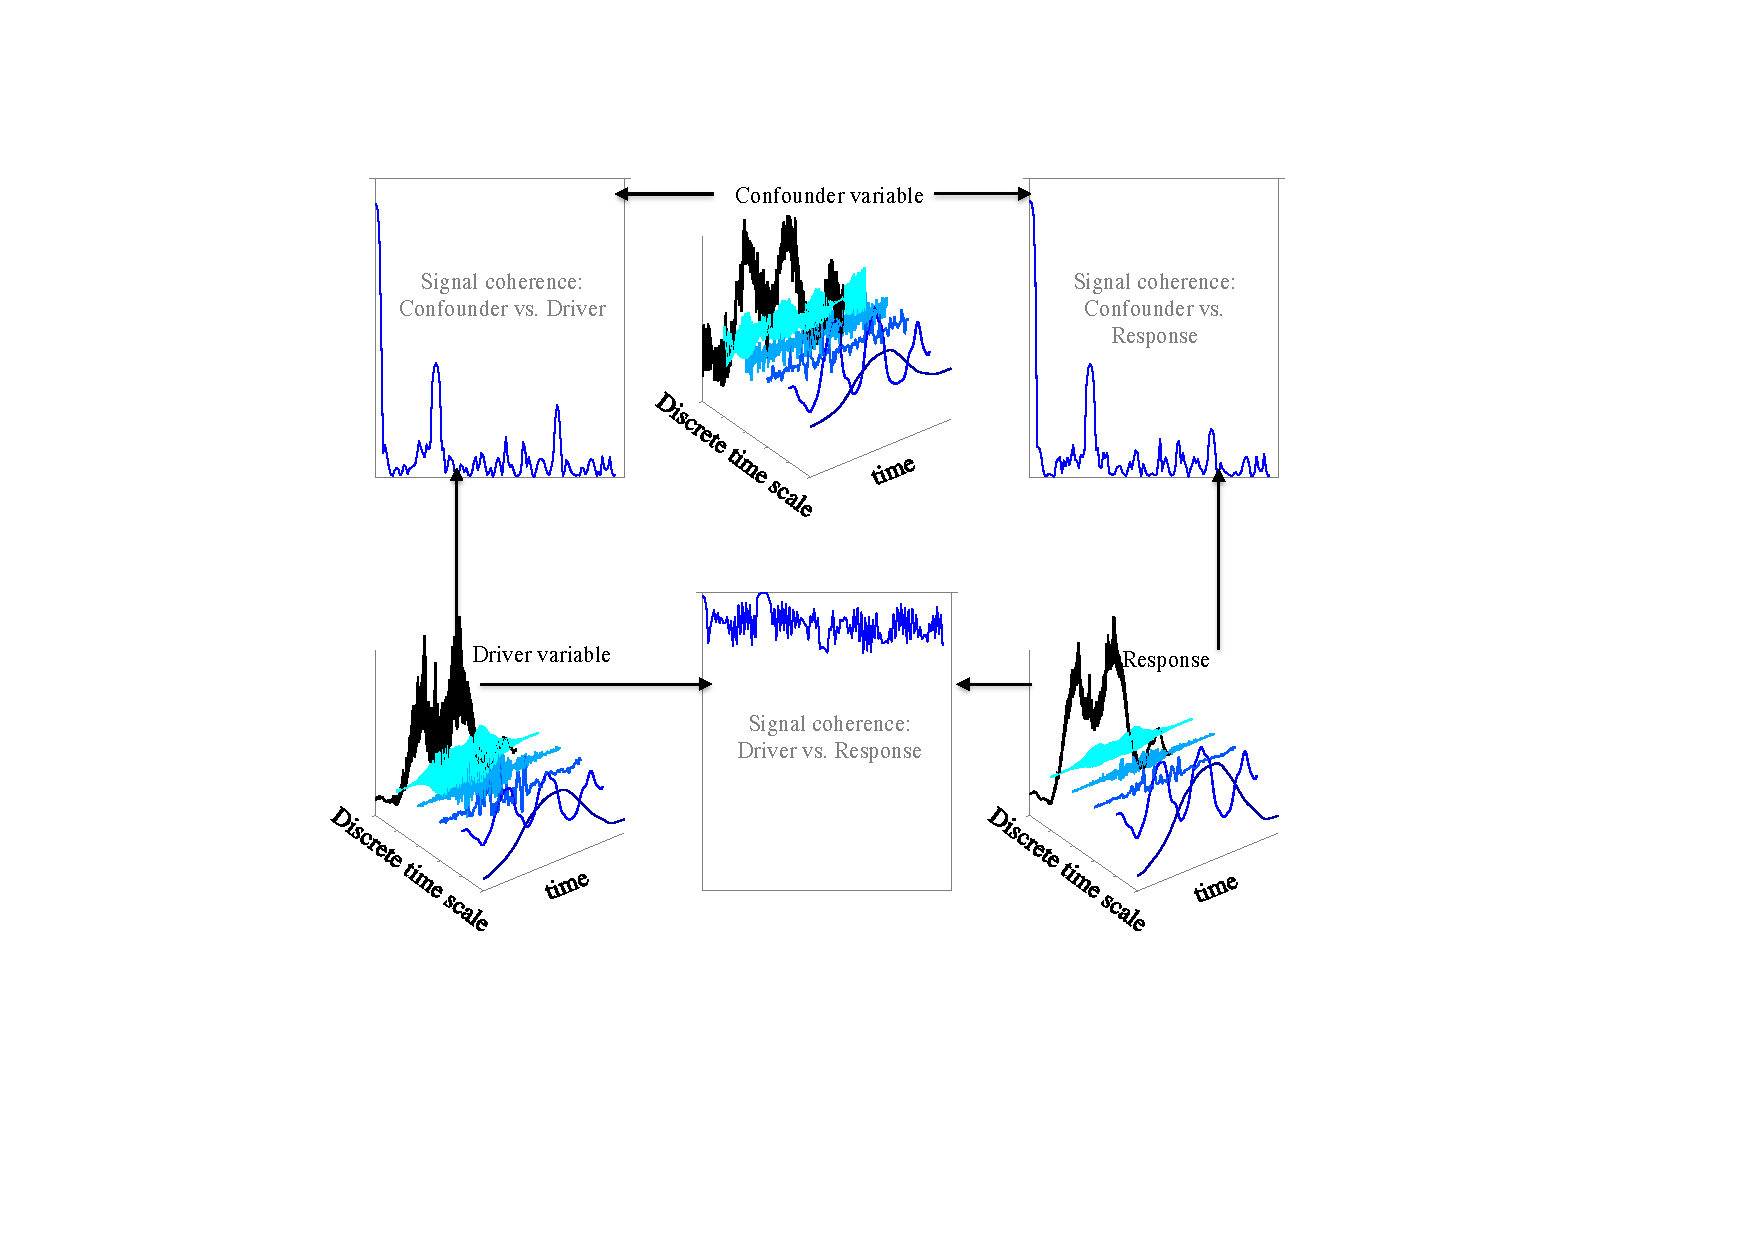
\includegraphics[width=.55\textwidth]{images/content/FIG1.pdf}
	\end{center}
	\end{figure}
\column{.2\textwidth}
\small{\textit{a pseudo caption}}
\vspace{4cm}
	\begin{figure}[tb]
		
\includegraphics[width=.6\textwidth]{images/qrcode-RSCAPE.jpg}
	\end{figure}
\end{columns}
\vspace{1cm}
We add some text here to show that the block will grow even over the bottom of the column. This demonstrates

						\vspace{3ex}
					\input{content/block_3a}
				}
			%\end{minipage}
		\end{center}
	\end{column}    
	% -------------
	% SECOND COLUMN
	% -------------
	\begin{column}{\mycolwidth}
		\begin{center}
			%\begin{minipage}[T]{.95\textwidth}
				\parbox[t][\columnheight]{\textwidth}{
					
% vim:set ff=unix expandtab ts=2 sw=2:
  {\vspace{.2cm}\textbf{REddyProc}\hfill\normalsize{A. Moffat, T. Wutzler, O. Menzer \& M. Migliavacca}}
\alert{\textit{Context:}}

\begin{itemize}
    \item Data from eddy covariance measurements are key to understand atmosphere ecosystem exchange fluxes.
    \item A standardized processing of the raw data is necessary to ensure comparability across sites.
    \item Site PIs will benefit from being able to process their data by using the easy-to-use R-package.
\end{itemize}
 

\begin{columns}
\column{.8\textwidth}
    \begin{figure}[tb]
    \begin{center}
        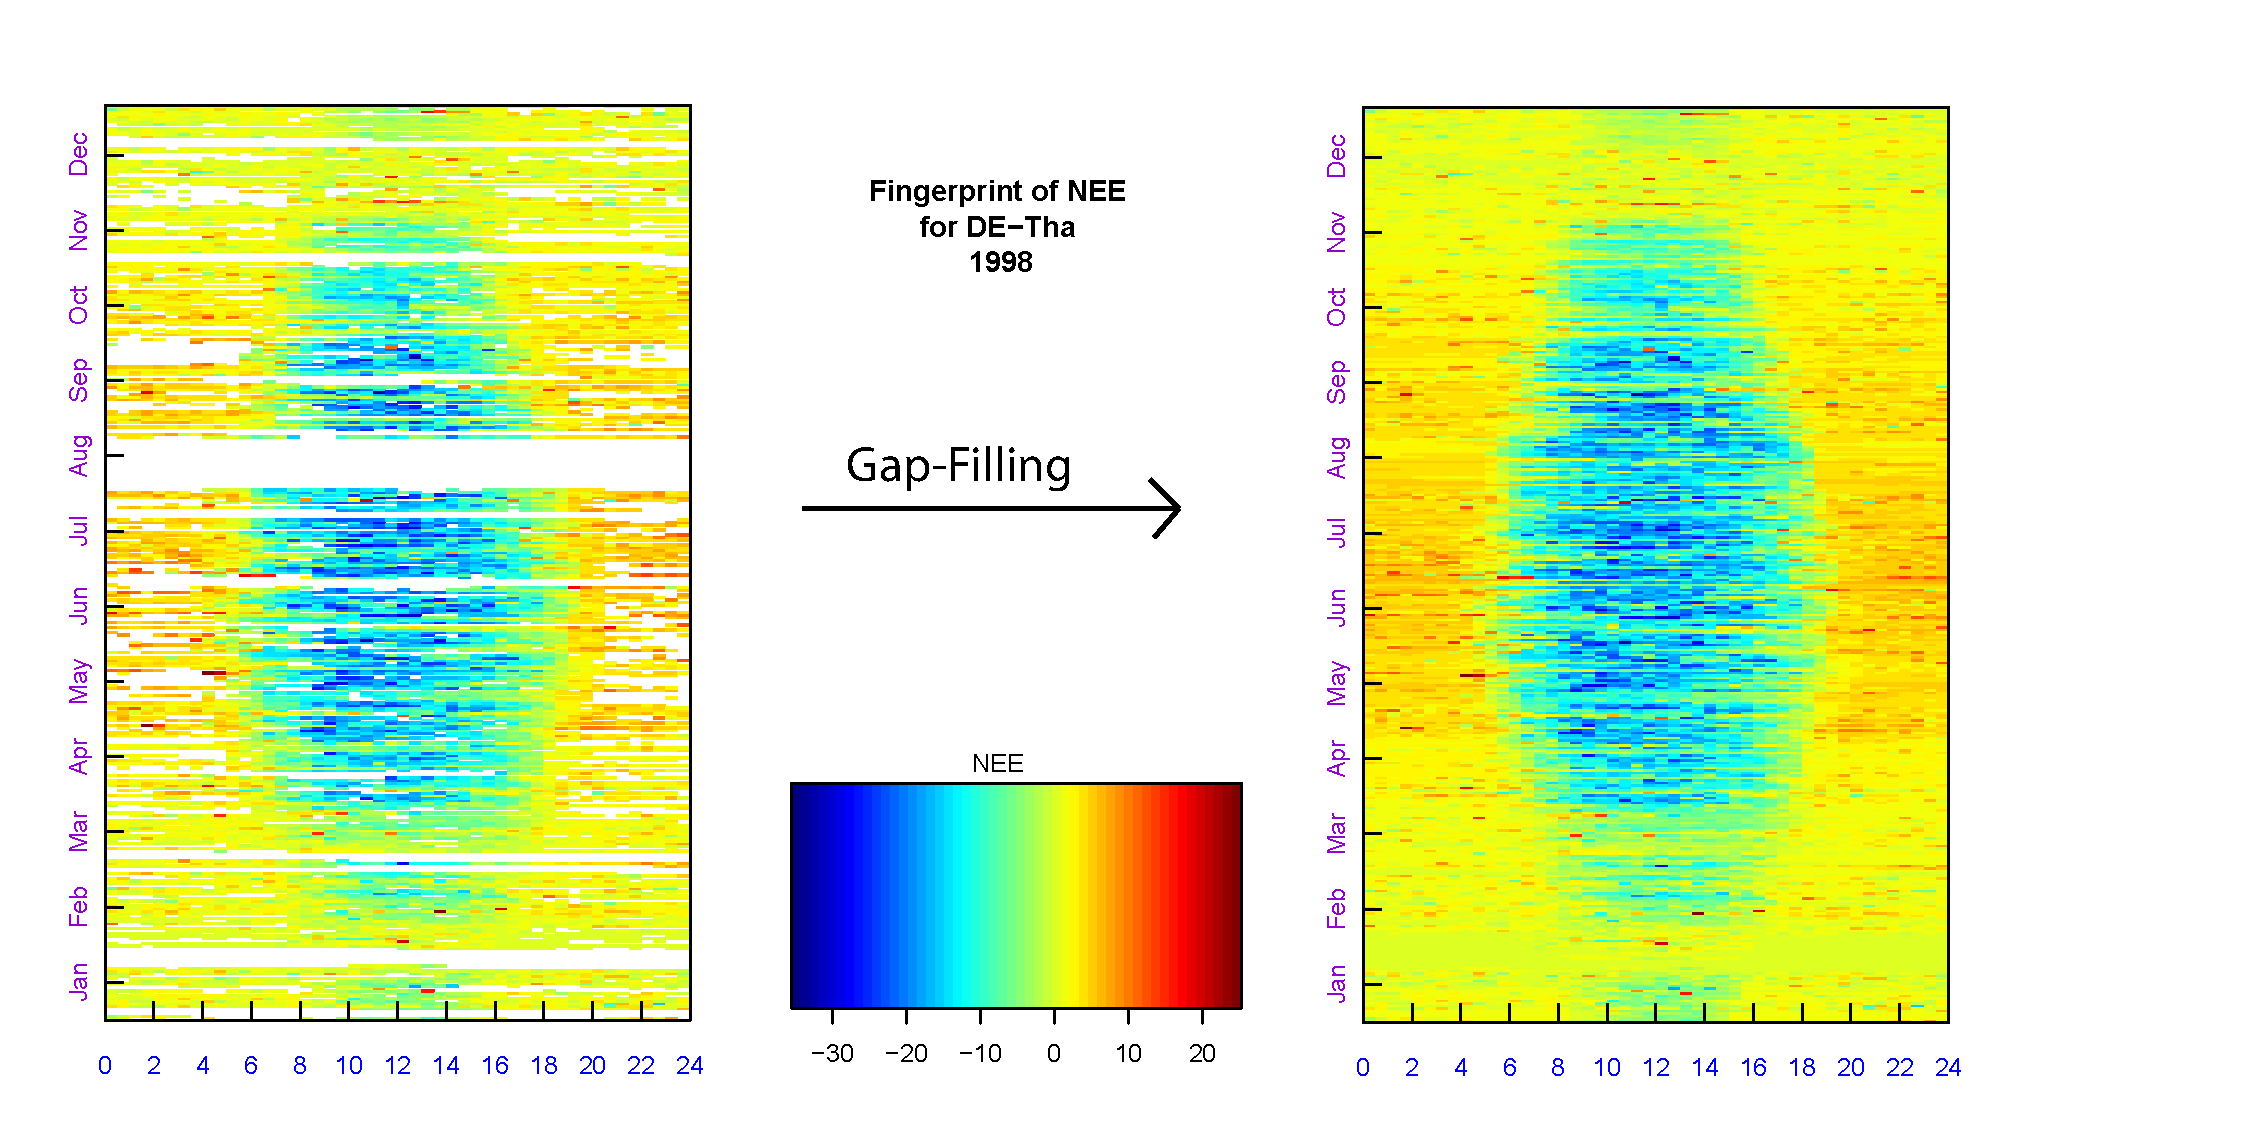
\includegraphics[width=.95\textwidth]{images/content/DE-Tha_1998_FP_NEE_ffc}
    \end{center}
    \end{figure}
\column{.2\textwidth}
\small{\textit{A fingerprint of ecosystem: Net ecosystem exchange (NEE) versus daytime and yearday}}
\vspace{4cm}
	\begin{figure}[tb]
		
\includegraphics[width=.6\textwidth]{images/qrcodeREddyProc.jpg}
	\end{figure}
\end{columns}
\vspace{1cm}
\hfill\large{\url{https://www.bgc-jena.mpg.de/bgi/index.php/Services/REddyProcWeb}}

					\vspace{3ex}
					
% vim:set ff=unix expandtab ts=2 sw=2:
{\textbf{RSCAPE}\hfill\normalsize{F. Gans \& M.D. Mahecha}}
\alert{\textit{Context:}}
\begin{itemize}
	\item Temperature is a key control of biogeochemical processes (e.g. on CO$_2$, CH$_4$, or N$_2$O production rates in soils)g.
	\item On seasonal and longer timescales other ecological factors e.g. substrate availability play an important role.
	\item The interaction of processes on different timescales is complicating the estimation of the temperature sensitivity of biogeochemcial processes.
\end{itemize}
 
\alert{\textit{Methods provided:}}
\begin{itemize}
	\item RSCAPE implements the "scale dependent parameter estimation” (SCAPE) principle (Mahecha et al. 2010).
    \item The user can choose amongst a wide range of 1) spectral decomposition methods and 2) standard or custom temperature sensitivity models.
    \item Full consideration to time-lagged responses and methodologcical uncertainties.
\end{itemize}
\vspace{1cm}
\begin{columns}
\column{.8\textwidth}
	\begin{figure}[tb]
	\begin{center}
		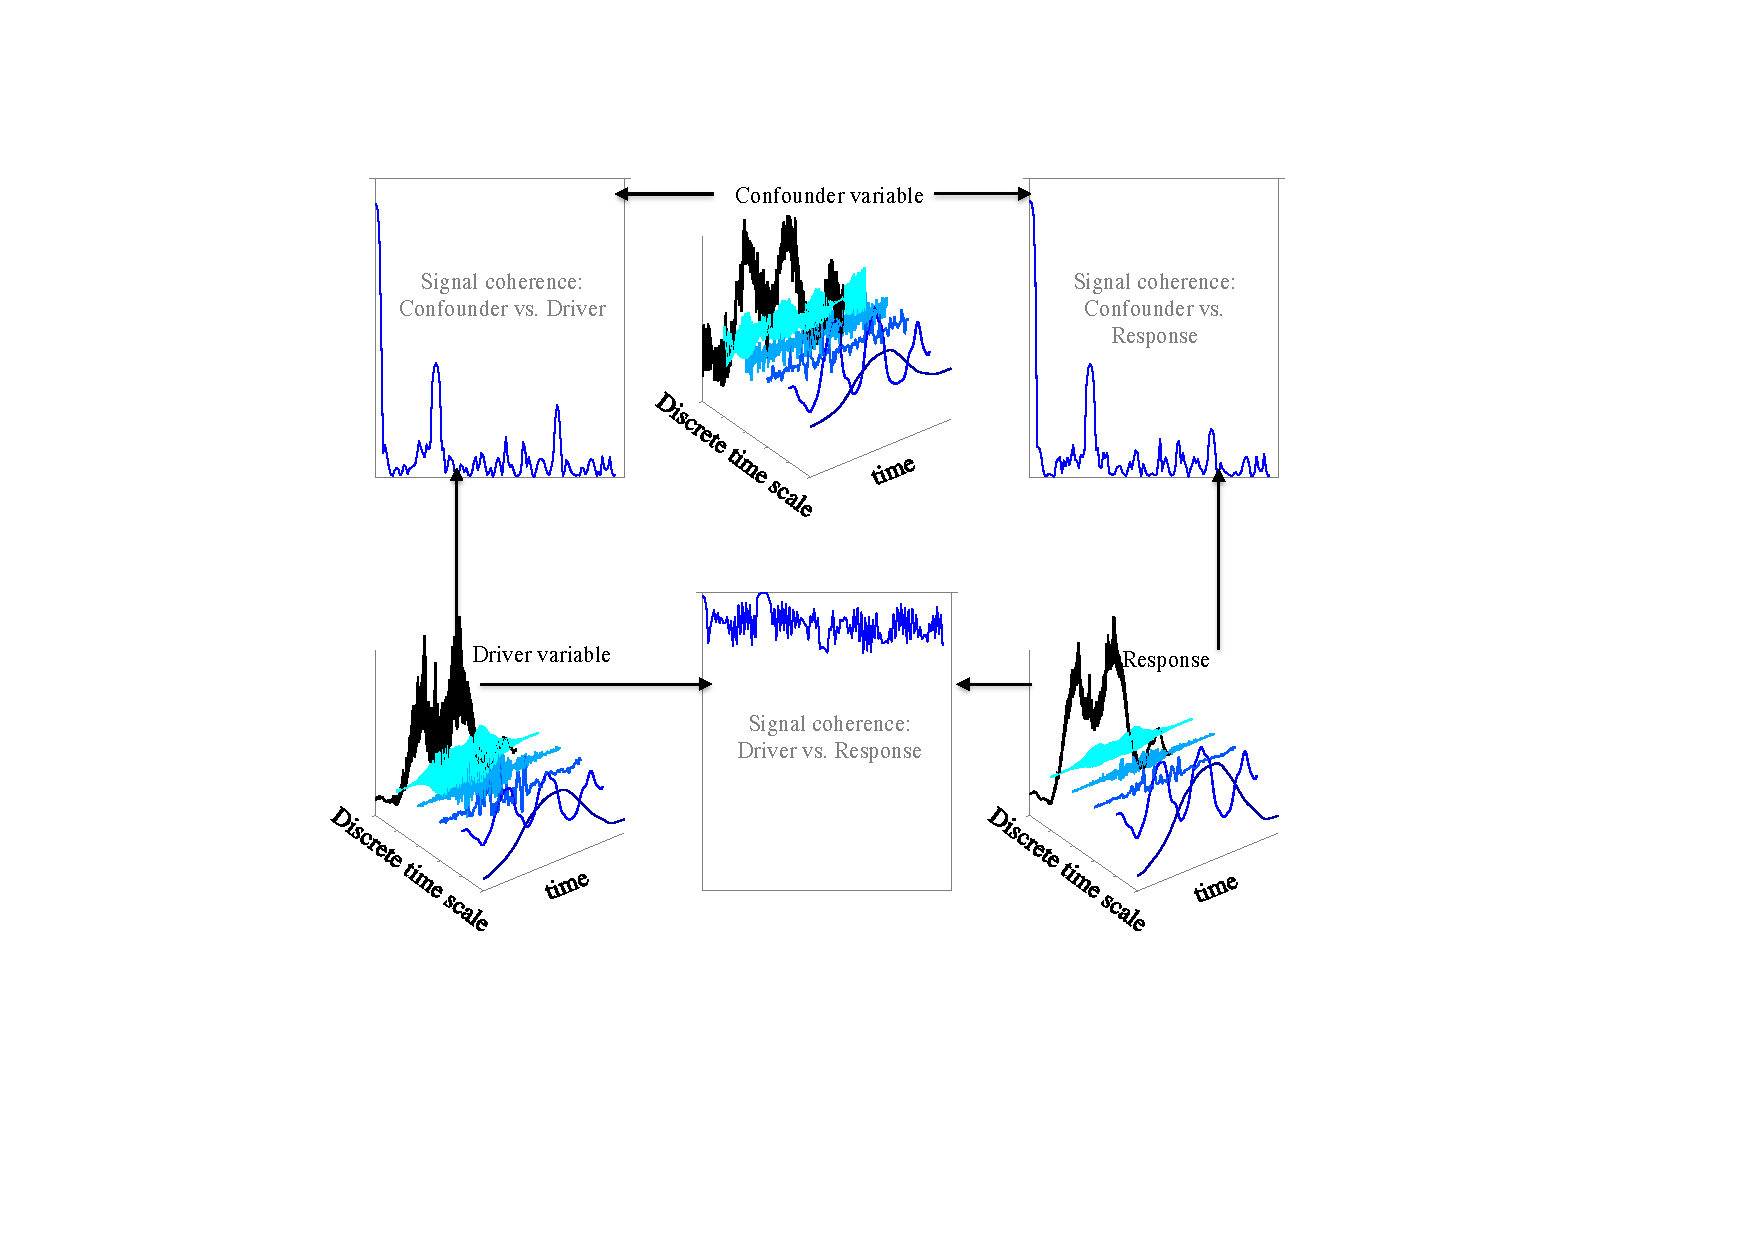
\includegraphics[width=.95\textwidth]{images/content/FIG1.pdf}
	\end{center}
	\end{figure}
\column{.2\textwidth}
\small{\textit{Conceptual problem solved by RSCAPE: The parameter estimtation problem (mapping from driver to response) is confounded on different time scales}}
\vspace{4cm}
	\begin{figure}[tb]
		
\includegraphics[width=.6\textwidth]{images/qrcode-RSCAPE.jpg}
	\end{figure}
\end{columns}
\vspace{1cm}
\hfill\large{\url{https://github.com/meggart/RSCAPE}}
\vfill

					\vspace{3ex}
					\input{content/block_3b}
				}
			%\end{minipage}
		\end{center}
	\end{column}    
	% -------------
	% THIRD COLUMN
	% -------------
	\begin{column}{\mycolwidth}
		\begin{center}
			%\begin{minipage}[T]{.95\textwidth}
				\parbox[t][\columnheight]{\textwidth}{
					
% vim:set ff=unix expandtab ts=2 sw=2:
  {\vspace{.2cm}\textbf{REddyProc}\hfill\normalsize{A. Moffat, T. Wutzler, O. Menzer \& M. Migliavacca}}
\alert{\textit{Context:}}

\begin{itemize}
    \item Data from eddy covariance measurements are key to understand atmosphere ecosystem exchange fluxes.
    \item A standardized processing of the raw data is necessary to ensure comparability across sites.
    \item Site PIs will benefit from being able to process their data by using the easy-to-use R-package.
\end{itemize}
 
\alert{\textit{Methods provided:}}
\begin{itemize}
    \item Filling gaps in the time series and providing uncertainties for the estimates.
\end{itemize}
\vspace{1cm}

\begin{columns}
\column{.8\textwidth}
    \begin{figure}[tb]
    \begin{center}
        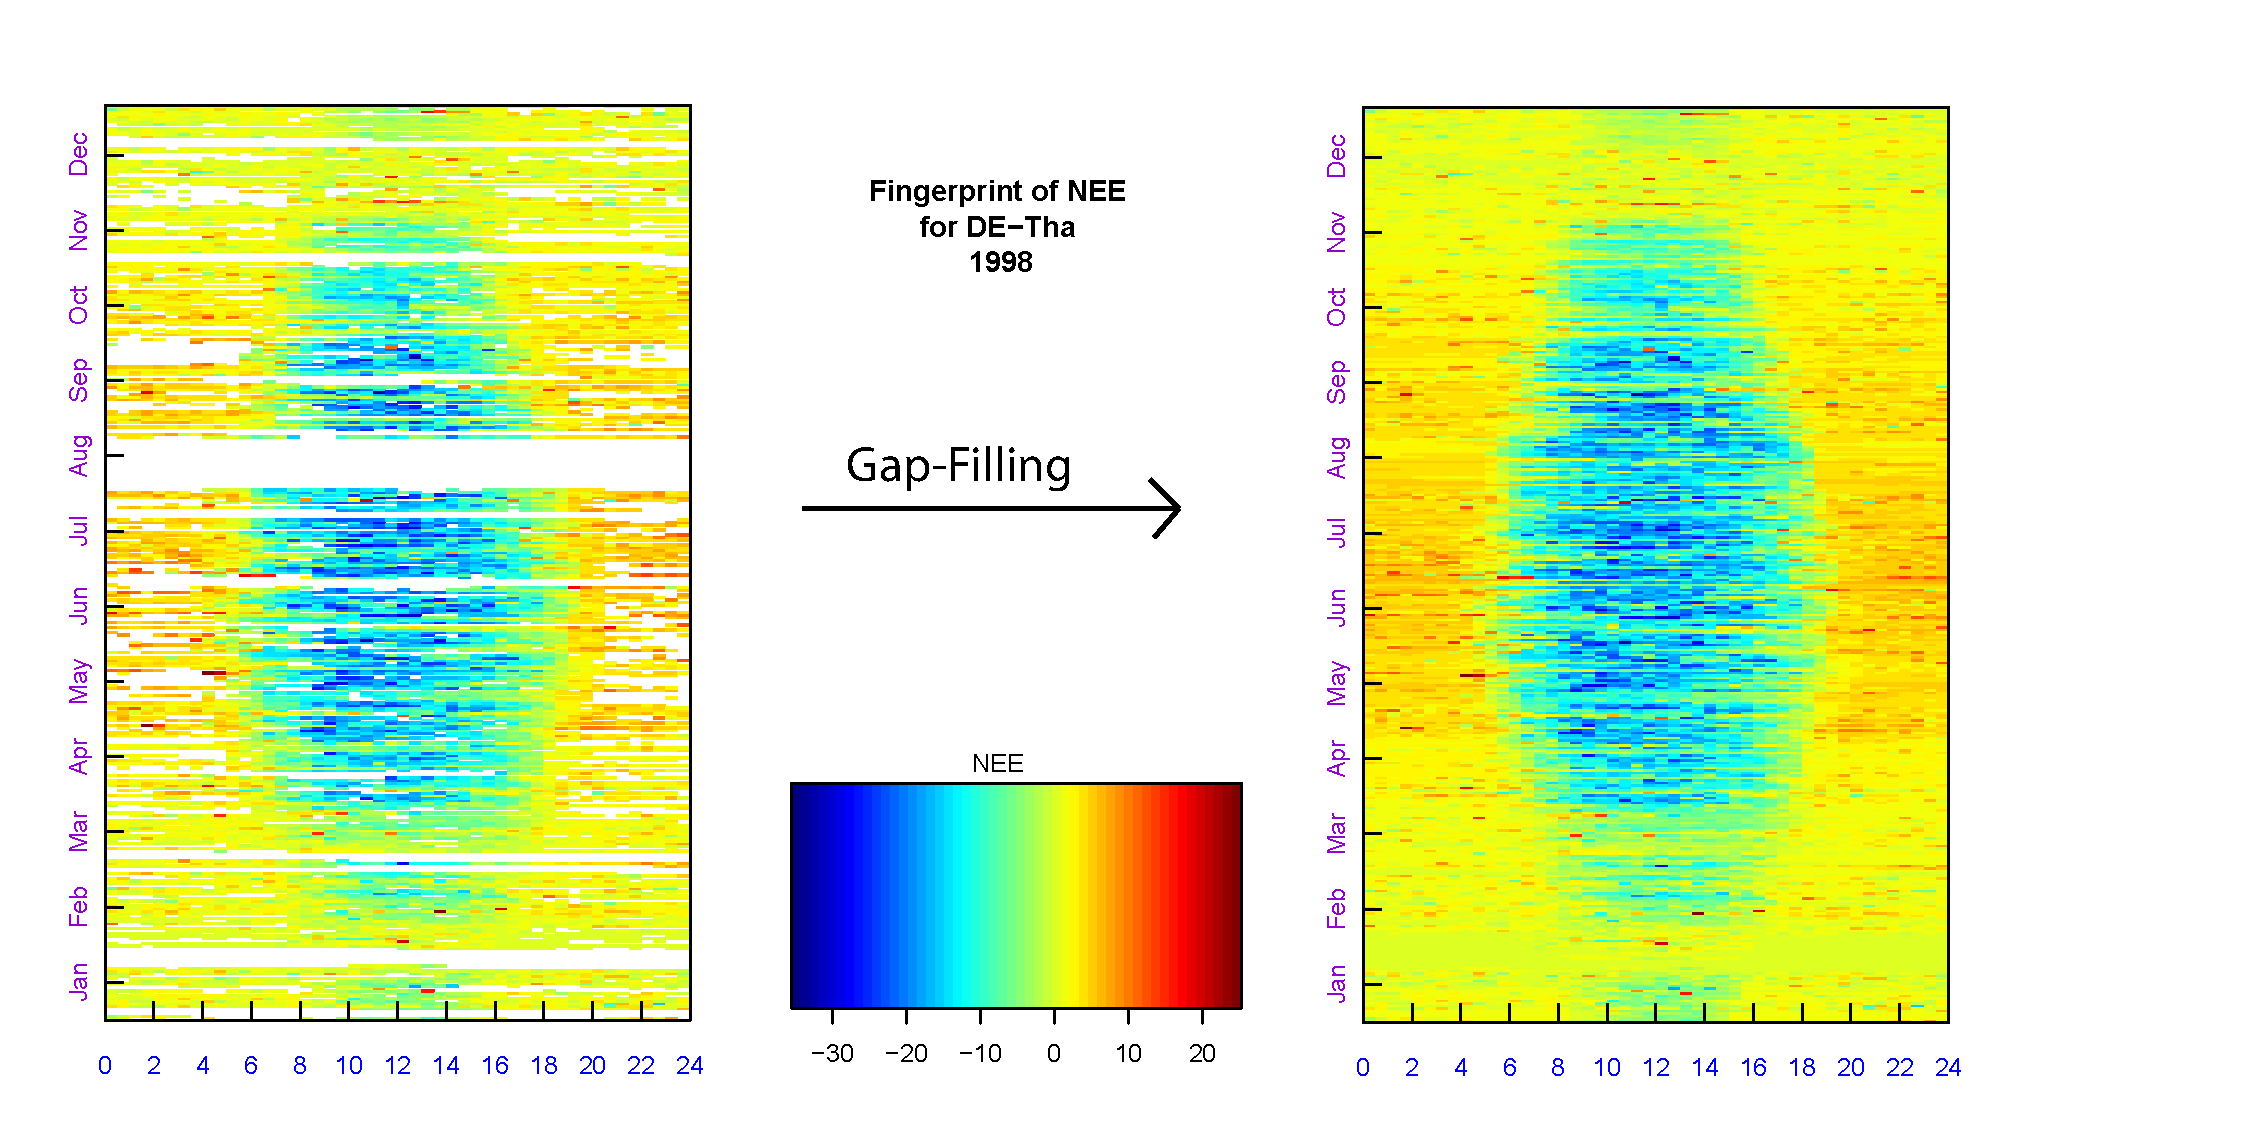
\includegraphics[width=.95\textwidth]{images/content/DE-Tha_1998_FP_NEE_ffc}
    \end{center}
    \end{figure}
\column{.2\textwidth}
\small{\textit{A fingerprint of ecosystem: Net ecosystem exchange (NEE) versus daytime and yearday}}
\vspace{4cm}
	\begin{figure}[tb]
		
\includegraphics[width=.6\textwidth]{images/qrcodeREddyProc.jpg}
	\end{figure}
\end{columns}
\vspace{1cm}
\hfill\large{\url{https://www.bgc-jena.mpg.de/bgi/index.php/Services/REddyProcWeb}}

					\vspace{3ex}
					
{\textbf{RSCAPE}\hfill\normalsize{F. Gans \& M.D. Mahecha}}
\alert{\textit{Context:}}
\begin{itemize}
	\item Temperature is a key control of biogeochemical processes (e.g. on CO$_2$, CH$_4$, or N$_2$O production rates in soils)g.
	\item The interaction of processes on different timescales is complicating the estimation of the temperature sensitivity of biogeochemcial processes.
\end{itemize}
 
\alert{\textit{Methods provided:}}
\begin{itemize}
	\item RSCAPE implements the "scale dependent parameter estimation” (SCAPE) principle (Mahecha et al. 2010).
\end{itemize}
\vspace{1cm}
\begin{columns}
\column{.8\textwidth}
	\begin{figure}[tb]
	\begin{center}
		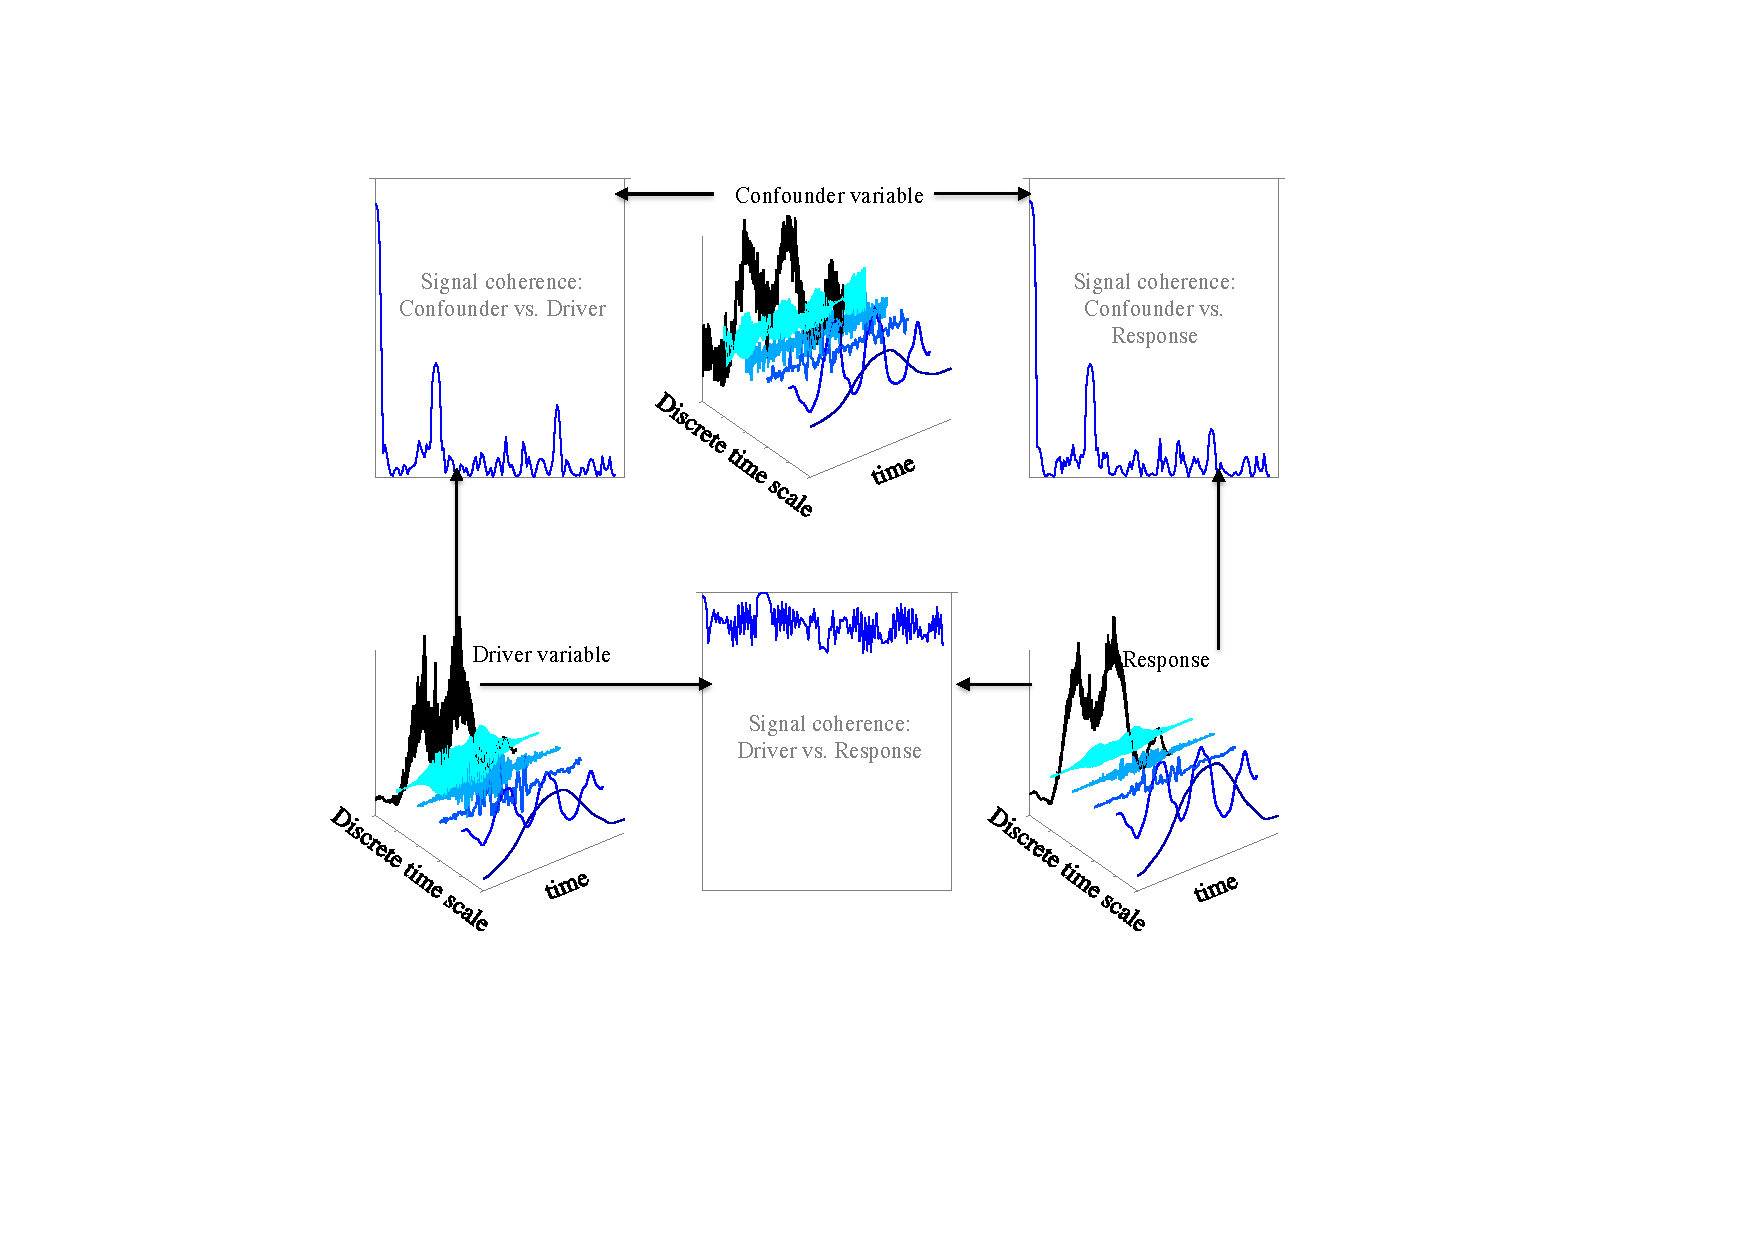
\includegraphics[width=.95\textwidth]{images/content/FIG1.pdf}
	\end{center}
	\end{figure}
\column{.2\textwidth}
\small{\textit{Conceptual problem solved by RSCAPE: The parameter estimtation problem (mapping from driver to response) is confounded on different time scales}}
\vspace{4cm}
	\begin{figure}[tb]
		
\includegraphics[width=.6\textwidth]{images/qrcode-RSCAPE.jpg}
	\end{figure}
\end{columns}
\vspace{1cm}
\hfill\large{\url{https://github.com/meggart/RSCAPE}}

					\vspace{3ex}
					\input{content/block_3c}
				}
			%\end{minipage}
		\end{center}
	\end{column}    



\end{columns}
